\documentclass{llncs}

\usepackage{graphicx}
\usepackage[hyphens]{url}
\usepackage{booktabs}
\usepackage{paralist}

% natbib for refs
%\usepackage[numbers,sort]{natbib} 

\begin{document}

\title{Popularity and
  Geospatial Spread of Immigration Trends on Twitter}

\author{Nabeel Albishry\inst{1,3}\thanks{This work has been supported by a doctoral research scholarship for
Nabeel Albishry from King Abdulaziz University, Kingdom of Saudi
Arabia.} \and Tom
  Crick\inst{2} \and Teleem Fagade\inst{1} \and Theo Tryfonas\inst{1}}


\institute{Faculty of Engineering, University of Bristol, UK\\\email{\{n.albishry,tesleem.fagade,theo.tryfonas\}@bristol.ac.uk}
\and 
Department of Computer Science, Swansea University, UK\\\email{thomas.crick@swansea.ac.uk}
\and
Faculty of Computing \& IT, King Abdulaziz University, Jeddah, Saudi Arabia\\\email{nalbishry@kau.edu.sa}}
\maketitle

\begin{abstract}
The techniques presented here helps giving broad understanding of
public concerns and common issue across different places. Hundreds of
topics trend throughout the day, which makes it nearly impossible to
analysis everything out there. Hence, the necessity of more generic
approach that is quick and less costly were main motivation behind the
work presented here. Therefore, all analysis and methods explained in
this paper are based on trends information only and do not include
processing of individual topics. With a year-worth of trends data,
this work investigates, popularity and geospatial spread of
trends. The findings show that spread likelihood of trend to other
places is, to some extent, influenced by the place at with it first
appeared. To the best of our knowledge, this is the first study to
address geospatial spread of trends on Twitter.
 \end{abstract}

\begin{keywords}
Trends, topic spread, network graphs, immigration, Twitter
\end{keywords}

\section{Introduction}\label{intro}

With the tremendous volume of tweets, trending topics serve as
valuable sources of information on summarising what is going on
Twitter, worldwide or in specific loca-tion. Apart from official trend
lists provided by the platform, on the website or through API
endpoints, trends and topics detection have been receiving a lot of
atten-tion across different research domains. In the health field for
example, monitoring and predicting of trending topics through social
media are adopted to measure health is-sues, such as flu spread, and
therefore have gained considerable attention in the recent years
[1]–[4]. Also, in marketing and business domain, topic detection and
classifica-tion are important approaches to extract knowledge about
public opinions from posts on social media [5], as well as in
analysing voting intentions and political view of users [6].

With the increasing popularity of social networks, effect of trends on
public have placed them in many social media campaigns and public
relations strategy. This has made trends a valuable target for
manipulation [7] stuffing [8], spamming [9][10] and hijacking
[11]. For example, the study in [12] explored a trend hijacking case
and suggested that increasing social media engagement may not be
beneficial for public relations.

A common approach in analysing Twitter trends is by clustering and
classification of trending topics based on content [13][14][15]. Also,
the study in [16] presented a content-independent method to model
trends progression through dynamics of users interactions. Other
studies aimed to provide real time classification or detection of
trends, such as [17][18]. With the increasing need for trends analysis
across various domains, customisable clustering tools that can be used
by non-technical users started to emerge, such as the recent example
introduced in [19].


\section{Methodology}\label{method}

\subsection{Context}

Before progressing to the methodology section, it is vital to briefly
present some statistics and information about the sample countries so
to clarify context boundaries.  Seven middle eastern countries were
selected for this study; Bahrain, Egypt, Ku-wait, Lebanon, Qatar,
Saudi Arabia, and United Arab Emirates (UAE). They include countries
with relatively big population (Egypt 97,553,000) and relatively small
pop-ulation (Bahrain 1,493,000) [20]. Kuwait was reported to have the
most daily active users [21]. As of March 2016, Saudi Arabia and Egypt
generate 33\% and 20\% of the Arab region tweets, respectively. Also,
Bahrain has the most balanced Arab country in terms of gender
breakdown of active users. Interestingly, between March 2014 and March
2016, Lebanon was the only country in the Arab states that has not
gained new active users, while UAE scored 60\%. Last but not least,
the GCC countries Bahrain, Kuwait, Qatar, UAE, and Saudi Arabia were
reported to have the highest penetration rate, respectively [21].

\subsection{Data Collection}

Trending topic lists in 7 countries were observed from 18th Oct 2016
until 31st Oct 2017. Every hour trending lists were collected through
Twitter REST API, which resulted in 7,948 hours' worth of records for
all the places, accumulating 2,307,163 trend records. It is important
to note that Twitter API does not necessarily have trends data
available for every request. For example, it is often to see no
information for tweet volume. For each country, list of available
trending topic is returned. From this list, four pieces of information
are extracted from each trend record:

\begin{itemize}
\item {\emph{woeid}}: The Yahoo! Where On Earth ID of the location;
\item {\emph{name}}: text of trending topic, such as `\#Call\_For\_Action';
\item {\emph{as\_of}}: recorded timestamp of the trend;
\item {\emph{tweet\_volume}}: volume of tweets over the past 24 hours, if it is available.
\end{itemize}

A note on volumes -- while the Twitter API returns list of trending
topic for a specific woeid place, their tweet volumes do not
accurately measure the tweeting activity in that place. Rather, tweet
volume refers to number of tweets containing the trend, re-gardless of
their place. Although Twitter documentation [22] does not provide any
further details on this, this conclusion was apparent after observing
trends that showed up in many places. Those trends were found with
same tweet volume across all places and, hence, participation volume
of each place was not possible to be accu-rately measured. Therefore,
the context of this study does not include any reference to this
volume entity.

\subsection{Graph Construction}

The paper utilises graph structures and their properties to conduct
analysis and results. The analysis approach involves constructing two
graphs; base graph that captures structure of trends raw data, and
aggregated graph which is computed from the base graph to unleash more
structures and hence additional
insights. Figure~\ref{fig:graphexamples} illustrates these
graphs. Nodes and direction orientation of edges are same in both
graphs. Therefore, nodes with zero indegree identify places, while
trend nodes feature zero outdegree.

\begin{figure}[htb]
\centering
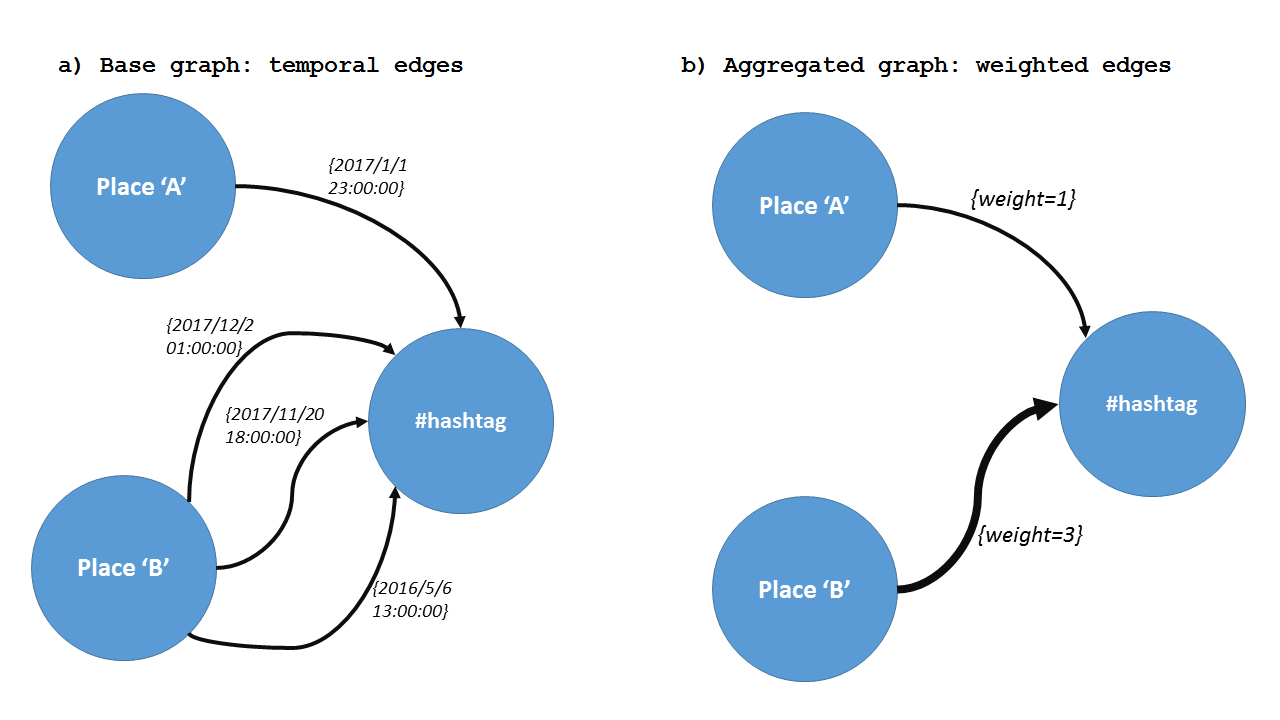
\includegraphics[width=\columnwidth]{images/graphexamples.png}
\caption{Graphs used in analyses}
\label{fig:graphexamples}
\end{figure}

{\textbf{Temporal base graph.}} This directed graph consists of three
trend entities: {\emph{place}}, {\emph{trend}} and
{\emph{timestamp}}. Nodes represent place and trends, and edges are
labelled with timestamps to indicate the time at which trend showed in
place. This graph is used to examine temporal properties, such as
spread.

{\textbf{Weighted aggregated graph.}} This graph combines temporal
edges between two nodes, in the base graph, into a single weighted
edge. The feature of weighted edges in this graph is used to measure
popularity of trends, repetition rate, participation of countries, and
volume of their participations.


\section{Results}\label{results}

Observation of the weighted graph provided overall evaluation of
activity for trends and places. In total there were 76,266 trend that
have trended 2,307,163 times across all places. This suggests that
trends may appear repeatedly over time. Overall repeti-tion ratio in
the dataset was 97\%, and ranged from 80\% to 98\% for individual
places, with Saudi Arabia scoring lowest and Qatar scoring highest
rate.

{\emph{Indegree}}, {\emph{outdegree}}, and {\emph{edges}} were used to
conduct subsequent results, further explanation is provided in due
course.


\subsection{Commonality and Popularity of Trends: weighted graph}

Node indegree indicates the number of places at which trend showed
(commonality), and weighted indegree is used to measure total number
of times a trend showed (pop-ularity). Indegree was used to group
trends to, while weighted indegree was used to analysis activity in
resulted groups, as shown in Table 1. Although 83\% of trends have
shown in one place only, their total weighted indegrees was about
41\%. In other words, there were less common trends amongst places,
but their popularity was higher than isolated trends\footnote{Isolated
trends are those that have trended in one place, i.e. their indegree
equal 1.}. This implies that trends showing across places do not
necessarily infer their activity or importance.

% TABLE 1 HERE

\subsection{Countries Participation: weighted graph}

Nodes outdegree reflects how many unique trends a place is connected
to (diversity), and weighted outdegree measures the ability of place
to generate trends (activity). Outdegree descriptive statistics,
presented in Table 2, shows that Saudi Arabia came at the top of the
list with 42\% of outgoing edges and weighing 20\% of total weight of
the graph. Closeness in the table shows how close a country node to
all other trend nodes. It shows that Saudi Arabia has connections to
56\% of trends in the graph. Nevertheless, interestingly Saudi Arabia
was found lowest in terms of maximum edge weight, mean and standard
deviation. On the other hand, Qatar was found with nearly total
opposite situation.

This can be read as that trends activity in Saudi Arabia was more
diverse and high in total, while more consistent. In contrast, Qatar
is connected to limited number of trends with more focused
activity. Also, Qatar’s outdegree is just 60\% of Bahrain’s, although
its weighted degree was 1.9 higher. 

% TABLE 2 HERE

\subsection{Edges Properties: weighted graph}

Edge weights in the graph were utilised to evaluate places activity in
indegree groups, shown in
Figure~\ref{fig:indegreegrouptrends}. Overall, most of places activity
went to common trends. Although Saudi Arabia was highest terms of
total activity, most of its activity, 61.26\% of its activity went to
isolated trends. Moreover, observing originating places for isolated
trends shows that about 30\% inbound edges came from Saudi Arabia, as
shown in Figure~\ref{fig:weightedcontributions}. Egypt contributed the
most in 2 and 3 indegree trend groups, United Arab Emirate in 4, 5 and
6 indegree trends, and for 7 indegree trends most in edges came from
Lebanon.

\begin{figure}[htb]
\centering
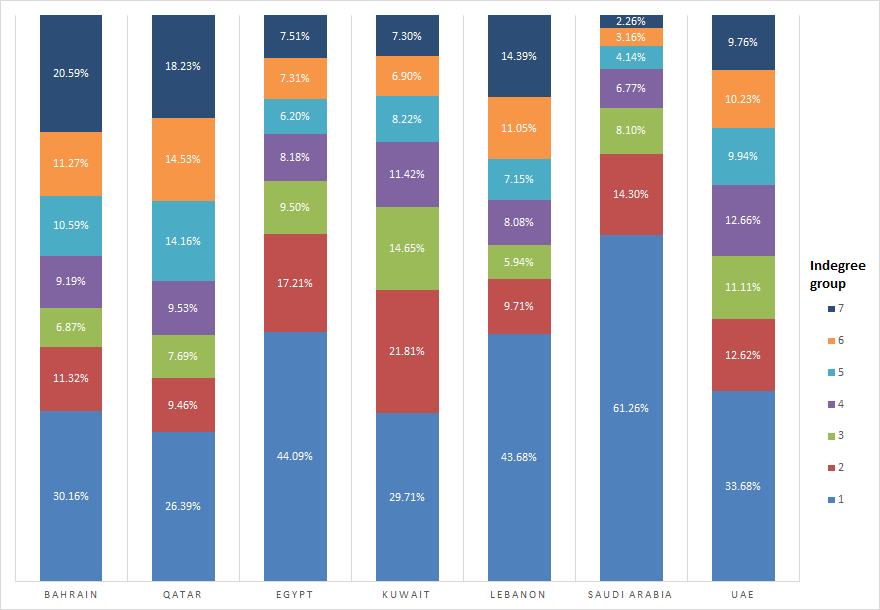
\includegraphics[width=\columnwidth]{images/indegreegrouptrends.png}
\caption{Trends Indegree group distributions across countries}
\label{fig:indegreegrouptrends}
\end{figure}

\begin{figure}[htb]
\centering
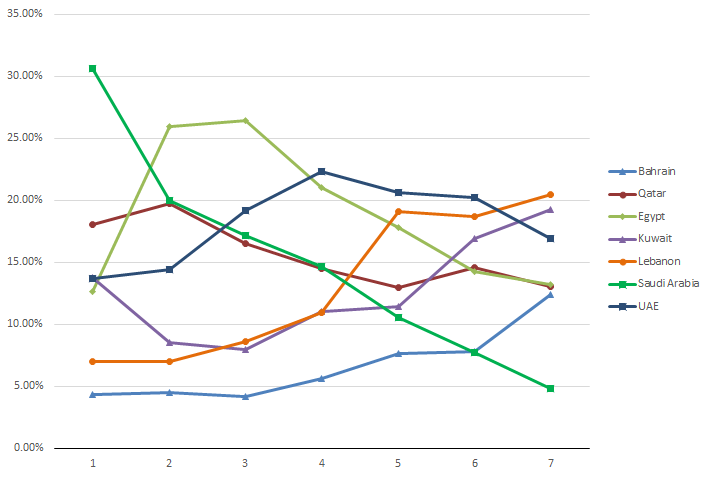
\includegraphics[width=\columnwidth]{images/weightedcontributions.png}
\caption{Weighted contribution of countries toward trends indegree groups}
\label{fig:weightedcontributions}
\end{figure}

\subsection{Temporal Spread and Reach}

As shown by Table 1, about 60\% of weighted indegree went to common
trends. To further examine temporal changes on those trends,
timestamps on in-edges of trend nodes in the temporal graph were
observed. Those timestamps were used to measure temporal order of
places for trend, as shown in Table 3. For instance, about 42\% of
first appearance of trends was in Saudi Arabia, while 36\% of 7th
trend appearance was in Bahrain.

% TABLE 3 HERE

Similar observation was made on outdegree measures, timestamps on
in-edges of place nodes in the temporal graph were observed. Results
are presented in Table 4. Highest portion of activities in Saudi,
Egypt and Lebanon made them 1st places for trends to appear
in. Nonetheless, Bahrain, UAE, Qatar, and Kuwait were more active with
trends that have appeared previously.

% TABLE 4 HERE

Additionally, reach of trend was measured to examine how many other
places a trend is likely to reach based on the country at which it
first appeared. Therefore, edges and related nodes relating to 1st
column in Table 3 were used. The results shown in Table 5 say that
62.3\% of trends that first appeared in Kuwait have also appeared in
one more place, and 5.1\% of those that first appeared in Qatar have
also appear in six more places.

% TABLE 5 HERE

Moreover, Table 6 shows origin of common trends grouped by their
indegree (connected places). As can be seen, 31.7.1\% of trends that
appeared in seven places have originated from Saudi Arabia, and 5\%
from Bahrain. Nevertheless, Bahrain was better in terms of further
reach.

% TABLE 6 HERE


\section{Discussion and Conclusions}\label{dissconc}

The results we can see that isolated trends were found most common
across coun-tries, although the study includes countries with high
share of active users and high tweets generation rate, like Saudi
Arabia and Egypt [21]. Also, number of trends returned by the API,
does not accurately reflect activity of place. Low trending topics may
indicate low consensus on discussed topics and does not necessarily
reflect tweeting activity. Also, number of trending topics is very
likely to include many repeated ones, and therefore high number of
trends does not necessarily imply more new topics. Furthermore, number
of trends was not found in correlation with tenden-cy of country to
participate in common trends. For example, Saudi Arabia was found
connected to 56\% of trends, however about 61\% them were isolated
trends, i.e. trends appeared only in Saudi Arabia. Meanwhile, most of
Qatar’s trends (73.6\%) were common ones, although it had edges with
6\% of trends. This indicates that activity of some places is more
focused on internal issues and concerns.

Also, further reach of trends (i.e. appearing in other places) was
observed for each place. Although a place may do well in reaching
other places, the number of trends it generates may affect total
reach. For example, Qatar was highest in reaching other places,
however it was the 5th in being the origin of trends that reach all
places. This was very clear in the case of Saudi Arabia. Its scores in
reaching other places were not as good as its scores in being the
origin of common trends, as shown in Table 5 and Table 6.

In conclusion, the study presented an approach to analyse trends data
using graphs and their properties. It shows the importance of graph
construction techniques to capture raw trends data that results in
temporal base graph. Then, it presents how aggregated weighted graph
can be generated from the base graph. The temporal graph was used to
measure temporal properties such as spread and reach. The weighted
graph was used to measures overall activities, such as commonality and
popularity of trends, and diversity and activity of places.

The presented approach showed how trends data can be used to evaluate
topics and places activity without the need to crawl individual
topics. Also, it shows how to measure spread of trends and reach based
on their historical records as well as the originating country.
 
The approach can be used and extended to identify trends of important
features. For example, to extract high spread trends, or how likely it
is for a trend to reach specific place from another one. 


% \begin{acks}
% This work has been supported by a doctoral research scholarship for
% Nabeel Albishry from King Abdulaziz University, Kingdom of Saudi
% Arabia.
% \end{acks}


% bib
\bibliographystyle{splncs}
\bibliography{iccci2018}

\end{document}
